
% vim:set ff=unix expandtab ts=2 sw=2:
\begin{multicols}{2}
The graphs show the reactions of a prototypical class of nonlinear two pool soil models to a disturbing time varying signal. 
This model is a technically simple place holder for ecologically motivated nonlinear systems like the soil models mentioned above to be analyzed in the future. It is given by:\\
\begin{eqnarray}
\dot{C}_x=I_{x}(t)  - \left(C_{x}^{2} + C_{x}\right) \operatorname{k_{x}}{\left (t \right )}\\
\dot{C}_y=I_{y}(t)  - \left(C_{y}^{2} + C_{y}\right) \operatorname{k_{y}}{\left (t \right )}
\end{eqnarray}
where $C_x,C_y$ are the carbon contents of two unconnected pools and the bounded  periodic functions $k_x(t) $ and $k_y(t) $ with:\\ 
\begin{eqnarray}
k_{x_{min}}\le  k_x(t) \le k_{x_{max}} \\k_{y_{min}} \le  k_y(t) \le k_{y_{max}}
\end{eqnarray}
describe the seasonal changes in decomposition speed.
e.g.:\\ 
\begin{eqnarray}
k_x=\frac{k_{xmax}}{2} + \frac{k_{xmin}}{2} + \frac{1}{2} \left(k_{xmax} - k_{xmin}\right) \sin{\left (4 t \right )}\\k_y=\frac{k_{ymax}}{2} + \frac{k_{ymin}}{2} + \frac{1}{2} \left(k_{ymax} - k_{ymin}\right) \sin{\left (4 t \right )}
\end{eqnarray}
The system can have a fixed point: 
$$ \mathbf{C}_f= \begin{pmatrix} C_{fx} \\ C_{fy} \end{pmatrix} $$
if the input streams have the same period and phase as the decomposition rates. For constant input streams it stays in a predictable region (an invariant set in the phase plane) \\ 
%\begin{eqnarray}
%\mathbf{I}_0(t)=\left(\begin{matrix}\left(C_{fx}^{2} + C_{fx}\right) \operatorname{k_{x}}{\left (t \right )}\\\left(C_{fy}^{2} + C_{fy}\right) \operatorname{k_{y}}{\left (t \right )}\end{matrix}\right)
%\end{eqnarray}
%The fixpoint would be.
%\[
%\mathcal{A}=\{\mathbf{C}_f\}
%\]
%We will now disturb both mass influxes individually by perturbations $u_x(t),u_y(t)$ and get: 
%\begin{eqnarray}
%\dot{C}_x=I_{0 x}(t) + u_{x}(t) - \left(C_{x}^{2} + C_{x}\right) \operatorname{k_{x}}{\left (t \right )}\\
%\dot{C}_y=I_{0 y}(t) + u_{y}(t) - \left(C_{y}^{2} + C_{y}\right) \operatorname{k_{y}}{\left (t \right )}
%\end{eqnarray}
The plots show the typical behavior of an ISS system: The changes in the state variables will asymptotically converge to a region of stability around an invariant set, whose size is a monotone function of the size of the disturbance (denoted by $|u|_{\infty}$).
For this particular system we proved the ISS property rigorously. The proof relies on the construction of an ISS Lyapunov function whose choice is \emph{not determined but  inspired} by a property of the system interpretable in ecologically terms. Expressed casually: "The  system can counteract supply changes fast enough".
This situation seems to be typical: The problem of establishing ISS for e.g. all the $\mathbf{I},\mathbf{T},\mathbf{N}$ models based on the ecologic principles they follow , is too hard.
But bio-chemical of biophysical restrictions could provide clues to ISS proofs for a particular system.
\\
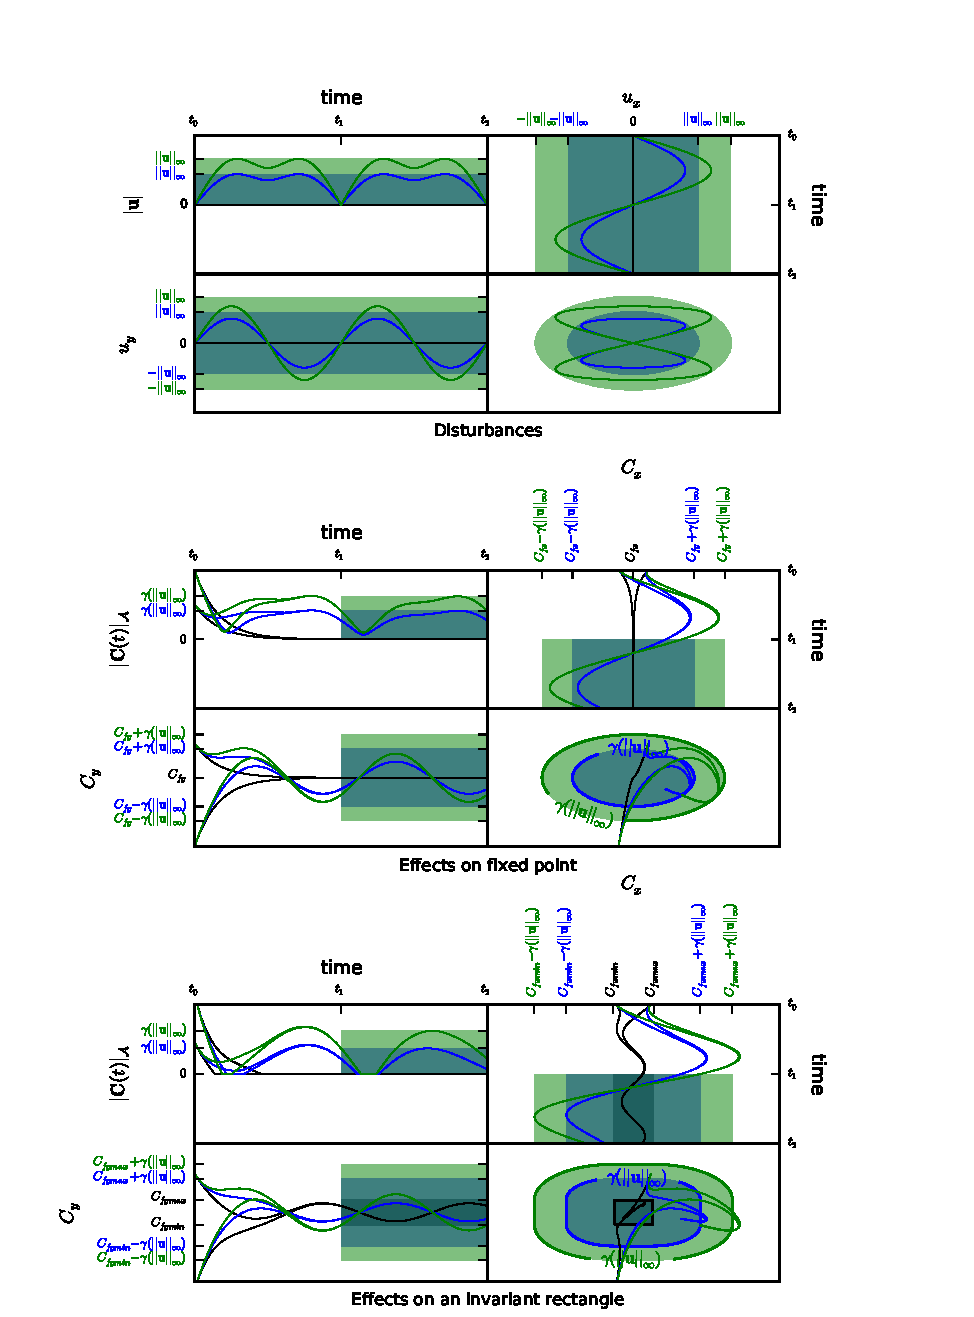
\includegraphics[width=\columnwidth]{combiPlot2.pdf}
\\
\begin{enumerate}
	\item
	The four plots on the top show the disturbances.
	\item
	The next four plots in the middle show the effect of this disturbances on the solutions for a system with fixed point. 
	\item
	The next four plots in the middle show the effect of this disturbances on the solutions for the system which no longer has a fixed point, but at least an invariant set, the dark blue square in the middle.
\end{enumerate}
\end{multicols}
